\documentclass[11pt]{article}

\usepackage{centernot}
\usepackage{amssymb}
\usepackage{xcolor}
\usepackage{verbatim}
\usepackage{multicol}
\usepackage{enumitem}
\usepackage{amsfonts}
\usepackage{amsmath}
\usepackage[utf8]{inputenc}
\usepackage[export]{adjustbox}  % for correct logo rendering
\usepackage{fancyhdr}  % for header/footer formatting
\usepackage{hyperref}  % for hyper-references
\usepackage{datetime}  % to update month in footer
\usepackage{array}  % more flexible tables
\usepackage[includeheadfoot,
            left=1in,
            right=1in,
            top=0.75in,
            bottom=0.75in,
            headheight=40pt]{geometry} % geometry needs to know headheight to correctly render the footer
\usepackage{tikz} % For drawing grid boxes

\definecolor{darkblue}{RGB}{0, 0, 139}
\definecolor{lightblue}{RGB}{173, 216, 230}

% desired format for footer
\newdateformat{monthyeardate}{%
  \monthname[\THEMONTH] \THEYEAR}

% set up header/footer
\pagestyle{fancy}
\fancyhf{}  % clear all headers/footers
\renewcommand{\headrulewidth}{0pt}  % remove header rule
\renewcommand{\footrulewidth}{0pt}  % remove footer rule

% set up header

\fancypagestyle{firstpage}{
    \fancyhead[L]{
    \vspace{0pt}
    \hspace{-8pt}
    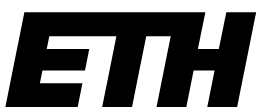
\includegraphics[width=0.1\textwidth]{docimgs/eth_logo_kurz_pos.png}\\
    \textbf{Swiss Federal Institute of Technology}\\
    \textbf{Zurich}\\
    %\textbf{ } \\
    
    }    

    \fancyhead[R]{
    \raggedleft
    %\vspace{20pt}
    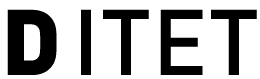
\includegraphics[width=0.13\textwidth]{docimgs/eth_ditet_logo_pos.png}\\
     \textbf{Dept. of Information Technology and} \\ \textbf{Electrical Engineering}  \\
     %\textbf{Chair for Mathematical Information} \\ \textbf{Information Science} \\

    }
}

% set up footer
\fancyfoot[L]{mdietz, ÜS 6}
\fancyfoot[C]{\thepage}
\fancyfoot[R]{\monthyeardate\today}

% set up section/subsection titles
\renewcommand{\thesection}{\arabic{section}}
\renewcommand{\thesubsection}{\arabic{subsection}}

% command used for simply emphasizing suggestions
\newcommand{\suggestion}[1]{{\itshape #1}}

%--- commands for transform arrows----------------
\newcommand{\transform}[2]{%
    \begin{tikzpicture}
        % Open circle
        \draw[thick] (0,0) circle (0.1);
        % Line with number above and adjustable length
        \draw[thick] (0.1,0) -- (#2,0) node[midway, above] {#1};
        % Filled circle
        \filldraw[thick] (#2,0) circle (0.1);
    \end{tikzpicture}%
}
\newcommand{\invtransform}[2]{%
    \begin{tikzpicture}
        % filled circle
        \filldraw[thick] (0,0) circle (0.1);
        % Line with number above and adjustable length
        \draw[thick] (0.1,0) -- (#2 -0.1,0) node[midway, above] {#1};
        % open circle
        \draw[thick] (#2,0) circle (0.1);
    \end{tikzpicture}%
}
\newcommand{\verticaltransform}[4]{%
    \begin{tikzpicture}
        % Open circle at the bottom with text below
        \filldraw[thick] (0,0) circle (0.1) node[below=3pt] {$#4$};
        % Vertical line with number on the left
        \draw[thick] (0,0.1) -- (0,#2 -0.1) node[midway, left] {#1};
        % Filled circle at the top with text above
        \draw[thick] (0,#2) circle (0.1) node[above=3pt] {$#3$};
    \end{tikzpicture}%
}
\newcommand{\verticalinvtransform}[4]{%
    \begin{tikzpicture}
        % Open circle at the bottom with text below
        \draw[thick] (0,0) circle (0.1) node[below=3pt] {$#4$};
        % Vertical line with number on the left
        \draw[thick] (0,0.1) -- (0,#2) node[midway, left] {#1};
        % Filled circle at the top with text above
        \filldraw[thick] (0,#2) circle (0.1) node[above=3pt] {$#3$};
    \end{tikzpicture}%
}

\begin{document}
\thispagestyle{firstpage}

\setlength{\headheight}{1 \baselineskip}  % accomodate header
\setlength{\parindent}{0pt}  % remove initial paragraph indent
\setlength{\parskip}{\baselineskip}  % add skip between paragraphs

\vspace*{-5px}
\section*{Übungsstunde 6}

\section*{Themenüberblick}
\begin{itemize} 
    \item \textbf{Analoge Lineare Systeme im Frequenzbereich:}
    \item[] Fouriertransformation: Definition, Eigenschaften und Beispiele
    \item[] Dualität der Fouriertransformation
    \item[] Plancherelsche Identität und Parsevalsche Beziehung
\end{itemize}

\section*{Aufgaben für diese Woche}
\vspace{-0.5cm}

\underline{\textbf{56}}, \underline{\textbf{57}}, 58, \underline{\textbf{59}}, \underline{\textbf{60}}, 61, \underline{\textbf{62}}, 63, \underline{\textbf{64}}, 65, \underline{\textbf{66}}\\
\vspace{-0.5cm}

Die \underline{\textbf{fettgedruckten}} Übungen empfehle ich, weil sie wesentlich zu eurem Verständnis der Theorie beitragen und/oder sehr prüfungsrelevant sind.

\vfill \null
\pagebreak

\section*{Analoge Lineare Systeme im Frequenzbereich}
\vspace*{-0.5cm}
\subsection*{Motivation}
\vspace*{-0.75cm}
\begin{center}
    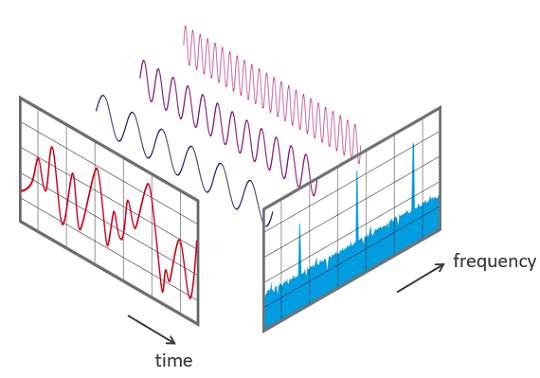
\includegraphics[width=0.35\linewidth]{docimgs/Zeit_und_Frequenzbereich.png}
    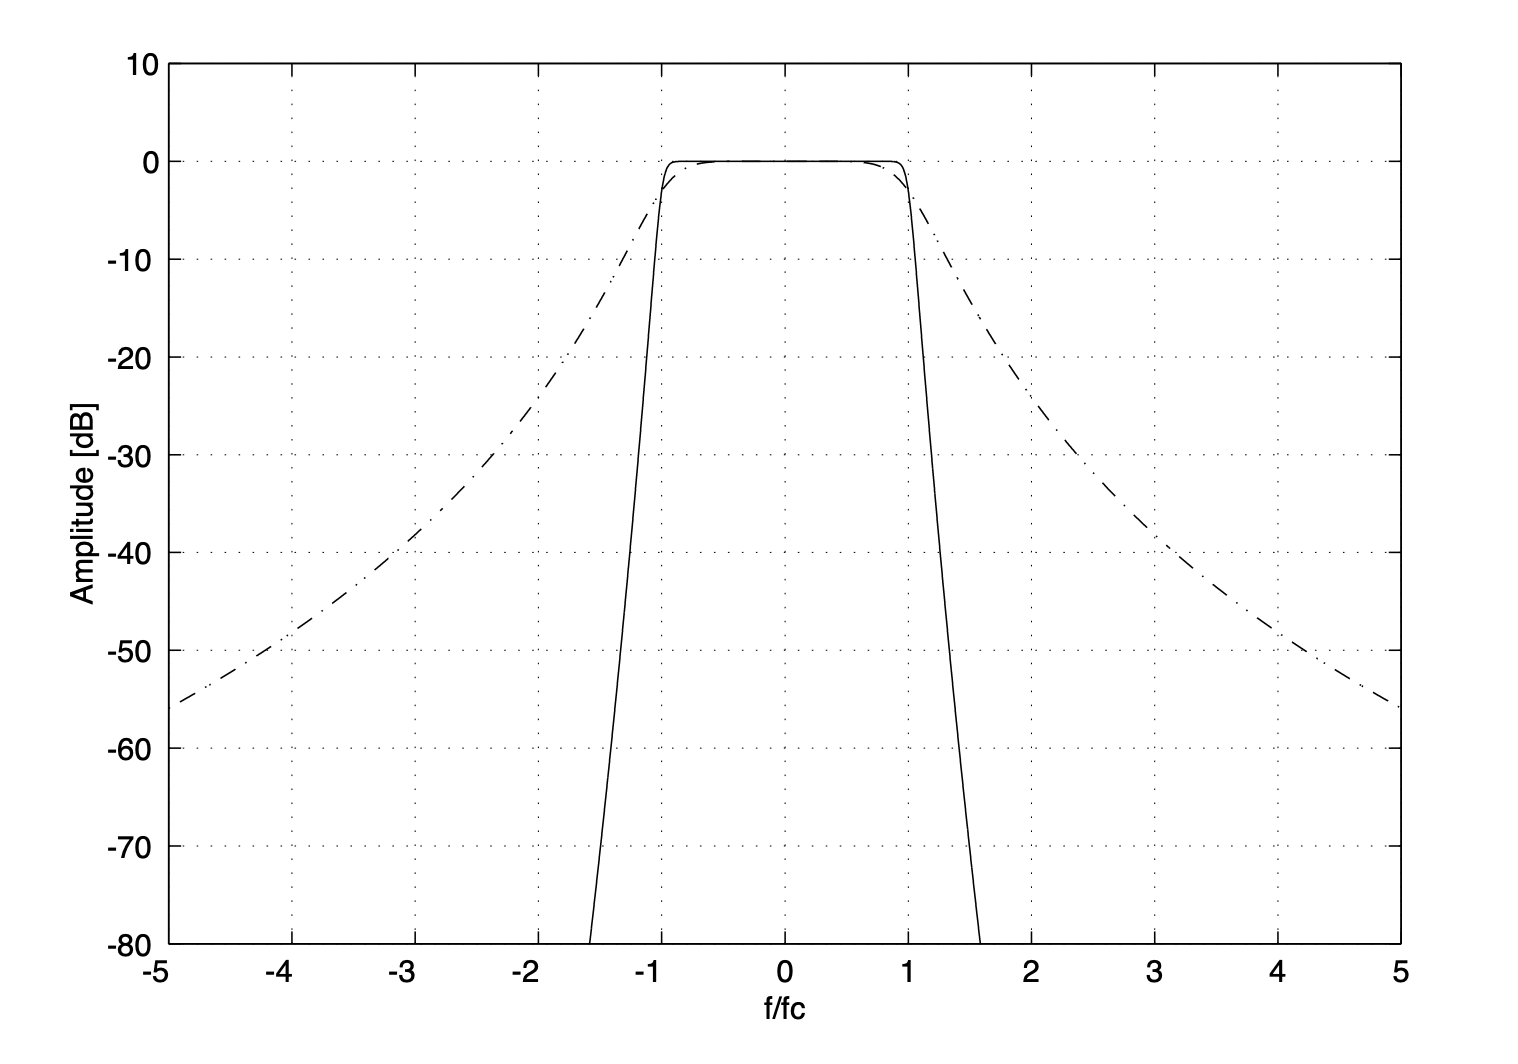
\includegraphics[width=0.3\linewidth]{docimgs/Butterworth_filter.png}
\end{center}
\vspace*{-0.5cm}
Das Frequenzspektrum ist ein mächtiges Werkzeug in SST1, da es wesentliche Eigenschaften von Signalen und Systemen offenbart, die im Zeitbereich verborgen bleiben. Wir können Signale in ihre Frequenzkomponenten zerlegen und somit Systeme für spezifische Aufgaben entwerfen und optimieren. Im Bereich der Signalverarbeitung ermöglicht das Frequenzspektrum effizientes Filtern, noise reduction und feature extraction. In der Kommunikationstechnik erleichtert es Modulation, Datenkompression und channel analysis für eine klarere Signalübertragung. In der Schaltungstheorie vereinfacht die Frequenzanalyse das Rechnen mit Wechselstromsignalen und hilft Ingenieuren, stabile und effiziente Schaltungen zu entwickeln. Diese Ansätze sind in vielen Bereichen grundlegend und liefern Einsichten und Lösungen, die durch eine reine Zeitbereichsanalyse nicht möglich wären.

\vspace*{-0.5cm}
\subsection*{Fouriertransformation}
\vspace*{-0.5cm}
\begin{itemize}[leftmargin=0pt]
    \item[] Die Fouriertransformation (FT) ist definiert durch:
    \item[] \fcolorbox{darkblue}{lightblue}{%
\parbox{\dimexpr\linewidth-2\fboxsep-2\fboxrule\relax}{
    $$\hat{x}(f) = (\mathcal{F}x)(f) = \int_{-\infty}^{\infty}x(t)e^{-2\pi i f t}\text{d}t$$
}}%
    \item[] Die dazugehörige Rücktransformation (IFT) ist dann:
    \item[] \fcolorbox{darkblue}{lightblue}{%
\parbox{\dimexpr\linewidth-2\fboxsep-2\fboxrule\relax}{
    $$x(t) = (\mathcal{F}^{-1}\hat{x})(t) = \int_{-\infty}^{\infty}\hat{x}(f)e^{2\pi i f t}\text{d}f$$
}}%
\item[] \textbf{Wichtiger Hinweis:} in KomA/NuS 2 war die Fouriertransformation und ihre Rücktransformation definiert als:
$$\hat{x}(\omega) = \int_{-\infty}^{\infty} x(t) e^{-i\omega t}\text{d}t, \hspace{20pt} x(t)=\frac{1}{2\pi} \int_{-\infty}^{\infty} \hat{x}(\omega)e^{i\omega t} \text{d}\omega$$
Da wir in SST1 $t$ und $f$ als Parameter haben anstatt $t$ und $\omega$, haben wir dank $\omega = 2\pi f $ und somit wegen $\text{d}\omega = 2\pi \text{d}f$ kein Vorfaktor $1/(2\pi)$ in der Rücktransformation.
\item[] Die Fouriertransformation ist eine \textbf{lineare Transformation}:
$$(\mathcal{F}(\alpha x_1 + \beta x_2))(f) = \alpha \hat{x_1}(f) + \beta \hat{x_2}(f) $$
\end{itemize}

\pagebreak

\subsection*{Riemann-Lebesgue Lemma}
\vspace*{-0.5cm}
Es sei $x$ ein absolut integrierbares Signal, d.h. $x \in L^1$.

Dann ist $(\mathcal{F}x)(f) = \hat{x}(f)$ stetig und $\displaystyle\lim_{|f| \to \infty} \hat{x}(f) = 0$.

\section*{Wichtige Beziehungen und Transformationspaare}
\vspace*{-0.5cm}

\subsection*{Verschiebung im Zeitbereich}
\vspace*{-0.5cm}
$x(t-t_0) \; \transform{2.}{1} \; e^{-2 \pi i f t_0} \hat{x}(f)$


\begin{tikzpicture}
    % Define the box size and grid spacing
    \draw[step=0.5cm,gray!50,very thin] (0,0) grid (16.5,3.5); % (0,0) is bottom-left corner, (10,10) is top-right corner
\end{tikzpicture}

\vspace*{-0.25cm}
Analog dazu gilt auch $e^{2\pi i f_0 t}x(t) \; \transform{3.}{1} \; \hat{x}(f-f_0) $

\subsection*{Faltung im Zeitbereich entspricht Multiplikation im Frequenzbereich}
\vspace*{-0.5cm}
$(x \ast y)(t) \; \transform{7.}{1} \; \hat{x}(f) \hat{y}(f)$


\begin{tikzpicture}
    % Define the box size and grid spacing
    \draw[step=0.5cm,gray!50,very thin] (0,0) grid (16.5,5.5); % (0,0) is bottom-left corner, (10,10) is top-right corner
\end{tikzpicture}

\vspace*{-0.25cm}
Analog dazu gilt auch $x(t)y(t) \; \transform{8.}{1} \; (\hat{x} \ast \hat{y})(f)$

\vfill \null
\pagebreak

\begin{center}
    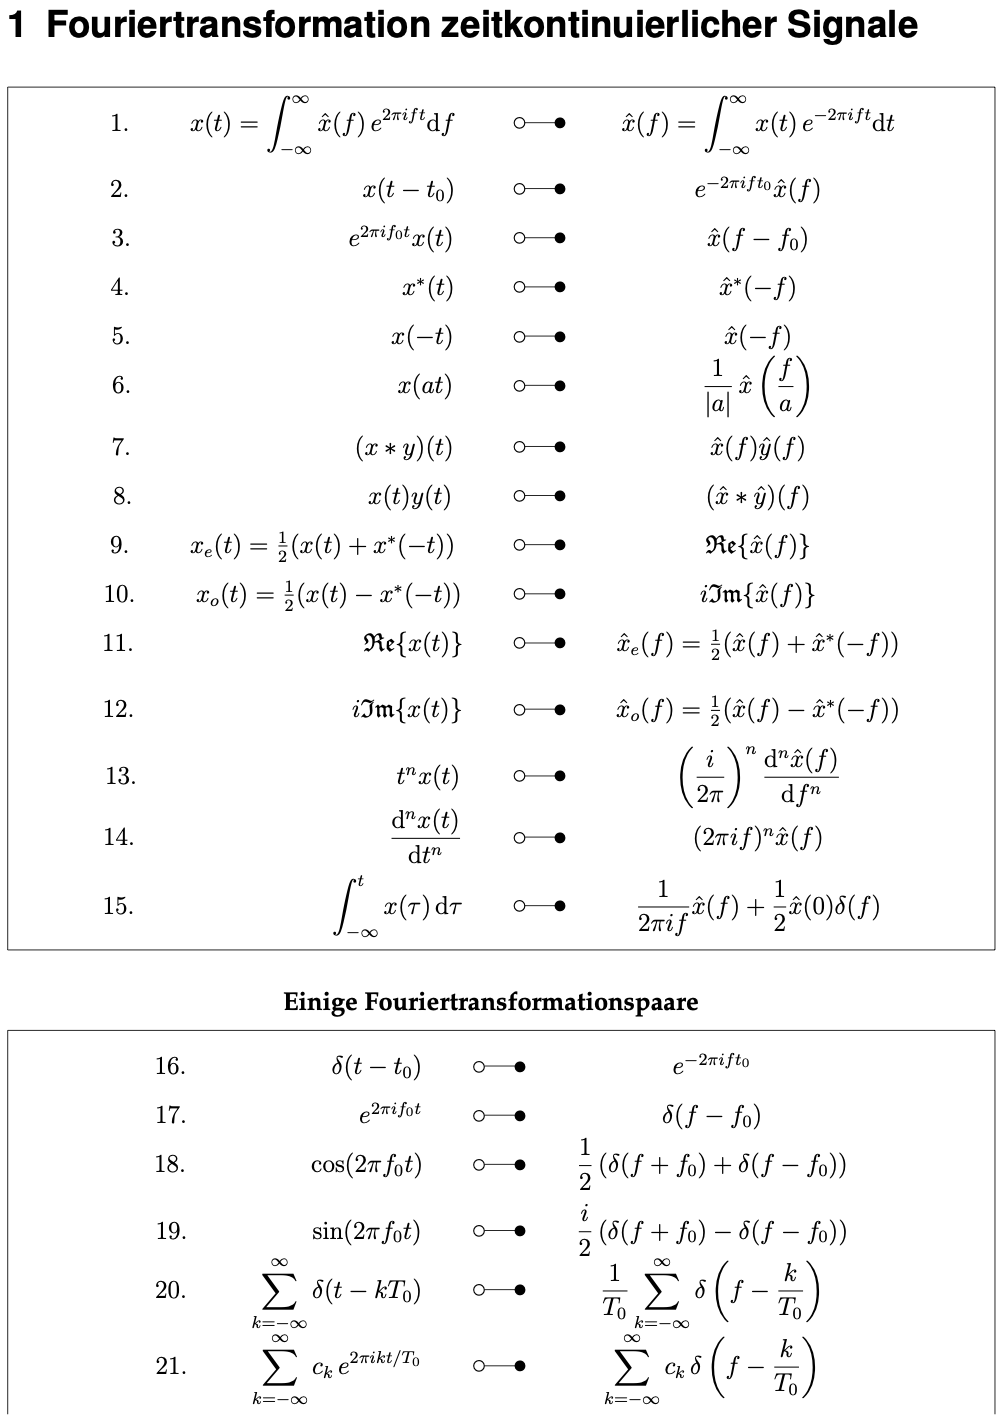
\includegraphics[width=0.85\linewidth]{docimgs/fs1.png}
\end{center}

\pagebreak

\begin{center}
    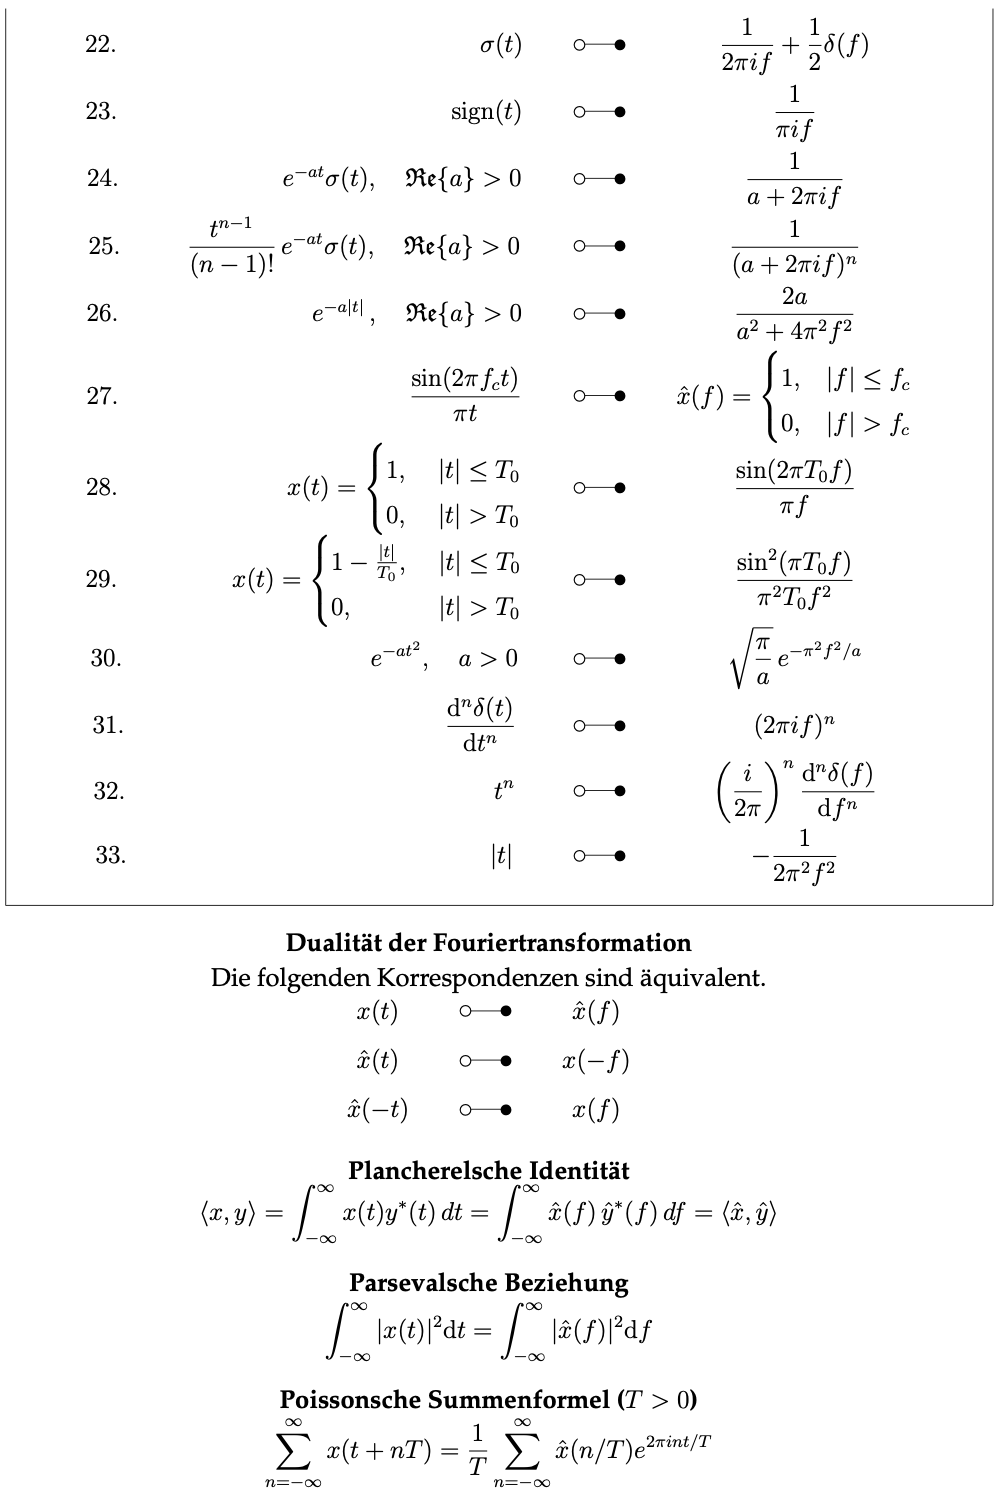
\includegraphics[width=0.85\linewidth]{docimgs/fs2.png}
\end{center}

\pagebreak

\subsection*{Aufgabe 58.b)}
\vspace*{-0.5cm}
Berechnen Sie die Fouriertransformierte der folgenden Signale:
\vspace*{-0.5cm}
\begin{itemize}
    \item[b)] $x(t) = \begin{cases}
        1 + \cos(\pi t), \hspace{13pt} |t| \leq 1\\
        0, \hspace{60pt} |t| > 1
    \end{cases}$
\end{itemize}


\begin{tikzpicture}
    % Define the box size and grid spacing
    \draw[step=0.5cm,gray!50,very thin] (0,0) grid (16.5,6
    ); % (0,0) is bottom-left corner, (10,10) is top-right corner
\end{tikzpicture}

\subsection*{Aufgabe 64}
Für die gegebenen Fouriertransformierten $\hat{x}(f)$ berechne man die zugehörigen Zeitsignale $x(t)$.
\vspace*{-0.5cm}
\begin{itemize}
    \item[b)] $\hat{x}(f) = \cos(8 \pi f + \frac{\pi}{3})$
\end{itemize}


\begin{tikzpicture}
    % Define the box size and grid spacing
    \draw[step=0.5cm,gray!50,very thin] (0,0) grid (16.5,6
    ); % (0,0) is bottom-left corner, (10,10) is top-right corner
\end{tikzpicture}

\pagebreak

\subsection*{Aufgabe 60}
\vspace*{-0.5cm}
Berechnen Sie die Fouriertransformierte der folgenden Signale:
\vspace*{-0.5cm}
\begin{itemize}
    \item[b)] $x(t)= te^{-2t} \sigma(t)$
    \item[c)] 
    \item[] \vspace*{-0.5cm}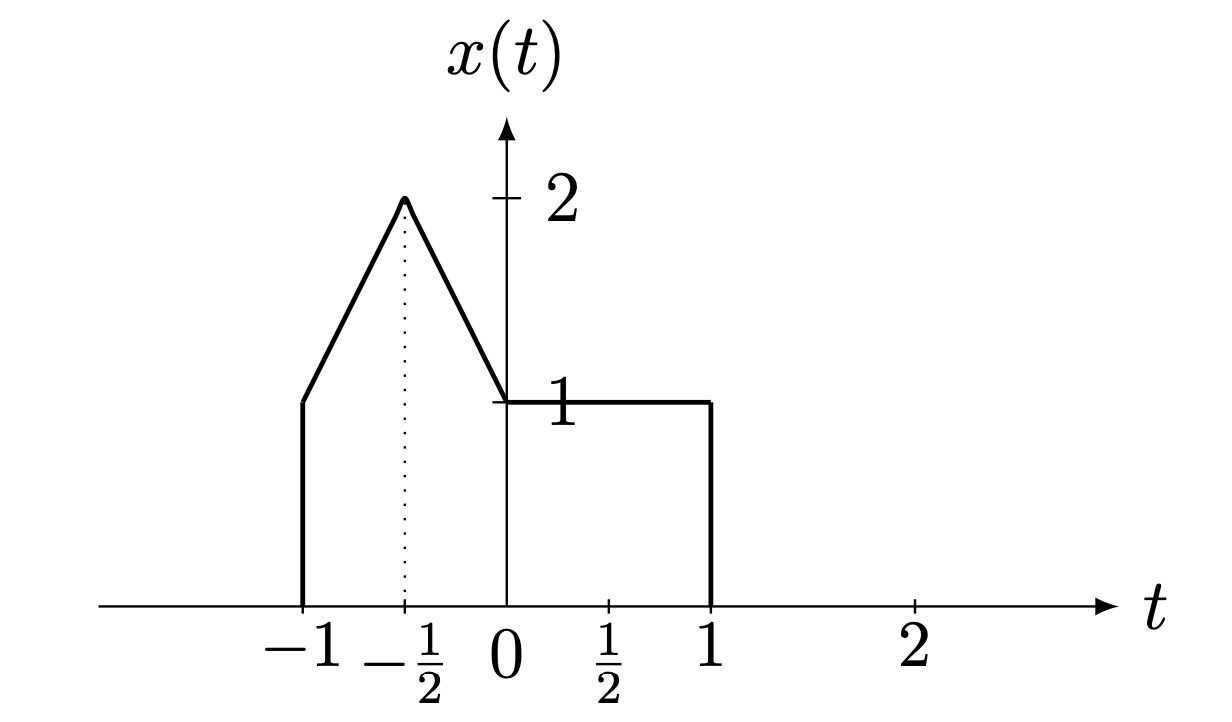
\includegraphics[width=0.4\linewidth]{docimgs/Aufgabe60.png}
\end{itemize}


\begin{tikzpicture}
    % Define the box size and grid spacing
    \draw[step=0.5cm,gray!50,very thin] (0,0) grid (16.5,12
    ); % (0,0) is bottom-left corner, (10,10) is top-right corner
\end{tikzpicture}

\vfill \null
\pagebreak

\section*{Weitere Zentrale Eigenschaften der Fouriertransformation}
\vspace*{-0.5cm}
\subsection*{Dualität der Fouriertransformation}
Man kann die Fouriertransformation als Rotation in der Zeit-Frequenz-Ebene betrachten:
\begin{multicols}{2}
    \includegraphics[width = 0.8\linewidth]{docimgs/dualität_1.png}
    \includegraphics[width = 0.8\linewidth]{docimgs/dualität_2.png}
\end{multicols}
Somit erhält die Fouriertransformationstabelle viel mehr Informationen als nur $x(t) \; \transform{}{1} \; \hat{x}(f)$
\begin{itemize}[leftmargin=0pt]
    \item[] \textbf{Beispiel}: In der Formelsammlung steht
    $$x(t) = \begin{cases}
        1-\frac{|t|}{T_0}, \hspace{12pt} |t| \leq T_0 \\
        0, \hspace{37pt} |t| > T_0
    \end{cases} \transform{29.}{2} \;  \frac{\text{sin}^2(\pi T_0 f)}{\pi^2 T_0 f^2}$$
    \item[] Wir suchen nun 
    $\mathcal{F}\left\{ \displaystyle\frac{\text{sin}^2(\pi f_0 t)}{\pi^2 f_0 t^2} \right\}(f)$, was wir jedoch nicht in der Formelsammlung finden können.
    \item[] Da aber $\hat{x}(t) \; \transform{}{1} \; x(-f)$ gilt, können wir die gewünschte Transformation wie folgt berechnen:
\end{itemize}


\begin{tikzpicture}
    % Define the box size and grid spacing
    \draw[step=0.5cm,gray!50,very thin] (0,0) grid (16.5,4
    ); % (0,0) is bottom-left corner, (10,10) is top-right corner
\end{tikzpicture}

\vfill \null
\pagebreak

\subsection*{Planscherelsche Identität und Parsevalsche Beziehung}
\vspace*{-0.5cm}
\begin{itemize}[leftmargin=0pt]
    \item[] Die beiden Beziehungen, um welche es in diesem Abschnitt geht, gehören meiner Meinung (und der Meinung vieler Mathematiker) nach, zu den wichtigsten und schönsten Eigenschaften der Fouriertransformation:
    \item[] \fcolorbox{darkblue}{lightblue}{%
    \parbox{\dimexpr\linewidth-2\fboxsep-2\fboxrule\relax}{
    \begin{center}
        \textbf{Plancherelsche Identität:}
    \end{center}
    $$\langle x, y \rangle = \int_{-\infty}^{\infty} x(t)y^\ast (t)\text{d}t = \int_{-\infty}^{\infty}\hat{x}(f)\hat{y}^\ast(f)\text{d}f = \langle \hat{x}, \hat{y} \rangle$$
    \begin{center}
        \textbf{Parsevalsche Beziehung:}
    \end{center}
    $$||x||^2 = \langle x, x \rangle = \int_{-\infty}^{\infty} |x(t)|^2\text{d}t = \int_{-\infty}^{\infty}|\hat{x}(f)|^2\text{d}f = \langle \hat{x}, \hat{x} \rangle = ||\hat{x}||^2$$
    }}
\end{itemize}
\vspace*{-0.5cm}
\subsection*{Parsevalsche Beziehung}
\vspace*{-0.5cm}
\begin{itemize}[leftmargin=0pt]
    \item[] Wenn wir zuerst die \textbf{Parsevalsche Beziehung} betrachten, können wir aus $||x||^2 = ||\hat{x}||^2$ schliessen, dass die Fouriertransformation eine Isometrie bezüglich der $L^2$-Norm, also eine längenerhaltende bijektive Transformation ist. 
    \item[] Man kann die Parsevalsche Beziehung sehr gut für die Berechnung der \textbf{Energie eines Signales} verwenden.
\end{itemize}
\vspace*{-0.5cm}
\subsection*{Plancherelsche Identität}
\vspace*{-0.5cm}
\begin{itemize}[leftmargin=0pt]
    \item[] Wenden wir uns nun der \textbf{Plancherelschen Identität} für Fouriertransformationen zu:
    \item[] \textbf{Theorem}: Wenn $x,y \in L^2(\mathbb{R})$, dann gilt $\langle x, y\rangle = \langle \hat{x}, \hat{y}\rangle$
    \item[] Somit ist die Fouriertransformation nicht nur längenerhaltend, sondern auch winkelerhaltend.
    \item[] \textbf{Beweis}:
\end{itemize}
\vspace*{-0.5cm}

\begin{tikzpicture}
    % Define the box size and grid spacing
    \draw[step=0.5cm,gray!50,very thin] (0,0) grid (16.5,4
    ); % (0,0) is bottom-left corner, (10,10) is top-right corner
\end{tikzpicture}
\vspace*{-0.5cm}
\begin{itemize}[leftmargin=0pt]
    \item[] Wenn wir nun in der Plancherelschen Identität $y = x$ wählen, so folgt daraus direkt die Parsevalsche Beziehung.
\end{itemize}

\pagebreak

\subsection*{Aufgabe 66}
\vspace*{-0.5cm}
Von einem Signal $x(t)$ ist die Fouriertransformierte gegeben als 
$$\hat{x}(f) = \begin{cases}
    1, \hspace{15pt} |f| \leq f_0\\
    0, \hspace{15pt} |f| > f_0
\end{cases}$$
Berechnen Sie die Energie des Signals $y(t) = \displaystyle\frac{\text{d}^2x(t)}{\text{d}t^2}$ gegeben durch
$$E_y = \int_{-\infty}^\infty |y(t)|^2 \text{d}t$$


\begin{tikzpicture}
    % Define the box size and grid spacing
    \draw[step=0.5cm,gray!50,very thin] (0,0) grid (16.5,4.5
    ); % (0,0) is bottom-left corner, (10,10) is top-right corner
\end{tikzpicture}

\subsection*{Sommer 2020 4.a)}
\vspace*{-0.5cm}
\begin{itemize}
    \item[$\star$] (a) (14 Punkte) Es sei $T \in \mathbb{R}_+, \; a \in \mathbb{R}$. Betrachten Sie das zeitkontinuierliche Signal
    $$x(t) = \cos(2 \pi t) + a \sin(2 \pi t), \hspace{12pt} t \in \mathbb{R},$$
    das gemäss
    $$y(t) = x(t)\sum_{n = - \infty}^{\infty} \delta(t-nT)$$
    abgetastet wird.
    \item[] \begin{itemize}
        \item[i.] (4 Punkte) Berechnen Sie das Spektrum $\hat{x}(f)$ des Signals $x(t)$.
        \item[ii.] (4 Punkte) Berechnen Sie das Spektrum $\hat{y}(f)$ des Signals $y(t)$.
        \item[iii.] (6 Punkte) Kann der Parameter $a$ für $T=1$ eindeutig aus $y(t)$ bestimmt werden? \textit{Hinweis: Betrachten Sie } $\hat{y}$.
    \end{itemize}
\end{itemize}

\vfill \null
\pagebreak


\begin{tikzpicture}
    % Define the box size and grid spacing
    \draw[step=0.5cm,gray!50,very thin] (0,0) grid (16.5,21
    ); % (0,0) is bottom-left corner, (10,10) is top-right corner
\end{tikzpicture}

\pagebreak

\subsection*{Prüfungsaufgabe: Sommer 2019, Aufgabe 2}

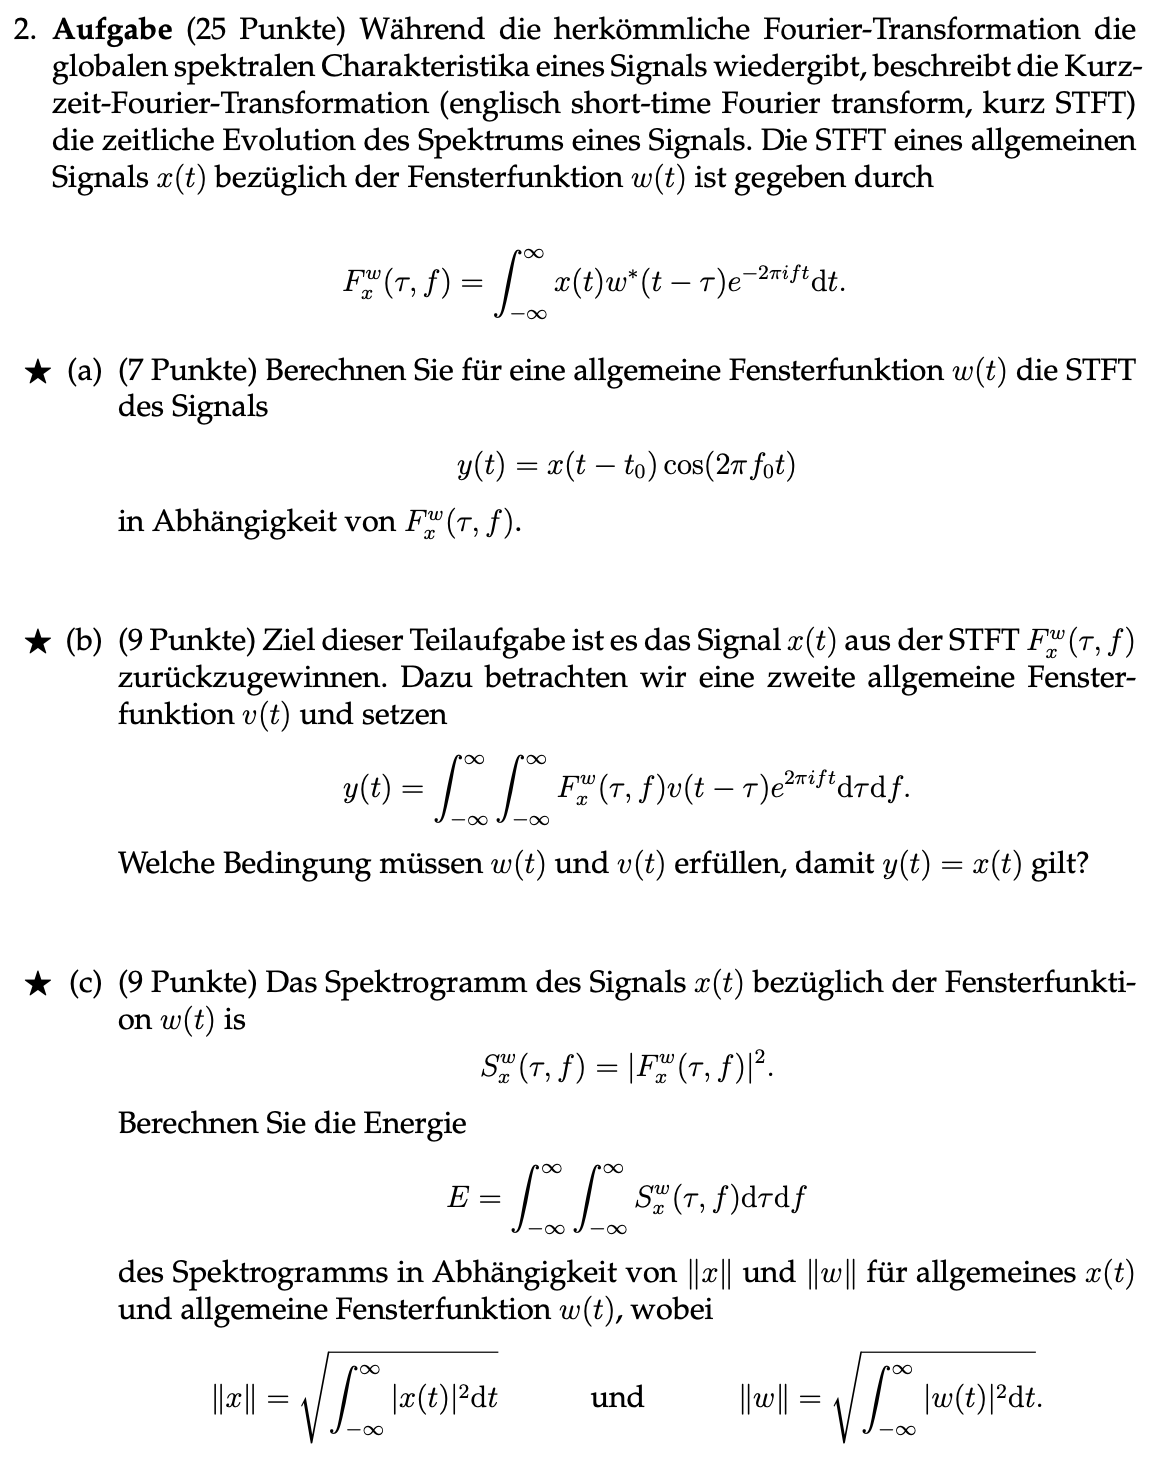
\includegraphics[width=0.9\linewidth]{docimgs/2019_ex2.png}


\vfill \null
\pagebreak


\begin{tikzpicture}
    % Define the box size and grid spacing
    \draw[step=0.5cm,gray!50,very thin] (0,0) grid (16.5,21
    ); % (0,0) is bottom-left corner, (10,10) is top-right corner
\end{tikzpicture}

\pagebreak


\begin{tikzpicture}
    % Define the box size and grid spacing
    \draw[step=0.5cm,gray!50,very thin] (0,0) grid (16.5,21
    ); % (0,0) is bottom-left corner, (10,10) is top-right corner
\end{tikzpicture}

\pagebreak


\end{document}
